As for the {\it water vapor transport}, studies of experimental data of concrete have indicated that permeability 
varies tremendously with temperature especially at temperature levels close to 100$^\circ$C. 
Introducing water vapor permeabilty as a scalar variable,
\begin{eqnarray}
\delta^{gw} = \frac{k^{rgw}k_{sat}}{\nu^{gw}} \quad ({\rm s}),
\end{eqnarray}
and denoting its maximum as $\delta_{wet}^{gw}$, the two possible diagrams of the water vapor permeability displayed 
in Fig.~\ref{s_shape} as a function of relative humidity  $RH = h$ and moisture content $w$, respectively, 
are plausible approximations of this dependence.
\begin{figure}[h!]
\begin{center}
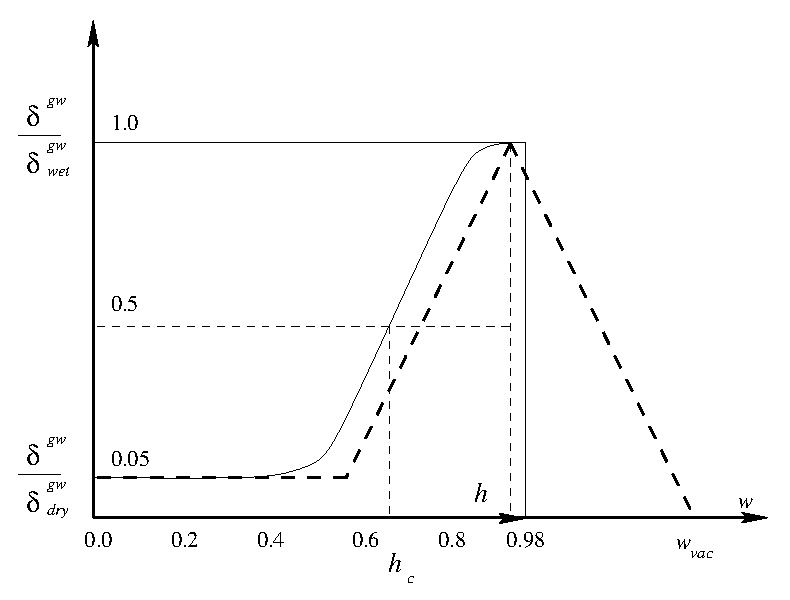
\includegraphics[angle=0, width=10cm]{PS/s_shape.eps}
\caption{Distribution of water vapor permeability as a function of $h$ and $w$}
\label{s_shape}
\end{center}
\end{figure}

\subsubsection{Bazant model}

\begin{center}
\begin{tabular}{|l|l|}
\hline
location & /TRFEL/SRC/bazped.cpp\\
         & /TRFEL/SRC/bazped.h
\\ \hline
related files &
\\ \hline
notes & 
\\ \hline
\end{tabular}
\end{center}

The solid S-shaped curve was proposed by Z. P. Ba\v{z}ant and L. J. Njjar in~\cite{bazant_n} using a function 
with three parameters $a_0$, $h_c$, $n$
\begin{equation}
\frac{\delta^{gw}}{\delta_{\rm wet}^{gw}} = a_0 + \frac{1 -a_0}{1 + \big(\frac{1 - h}{1 - h_c}\big)^n},
\end{equation}
where parameter $h_c$ characterizes the relative humidity at which $\delta^{gw}/\delta_{wet}^{gw}$ drops half-way between 
its maximum and minimum values. The dashed line was considered by \cite{pedersen}.


\subsubsection{Pedersen model}

\begin{center}
\begin{tabular}{|l|l|}
\hline
location & /TRFEL/SRC/pedersen.cpp\\
         & /TRFEL/SRC/pedersen.h
\\ \hline
related files &
\\ \hline
notes & 
\\ \hline
\end{tabular}
\end{center}

The dashed line was considered by \cite{pedersen}:
\begin{equation}
\delta^{gw} = \delta^{gw}_{\rm dry} + \frac{h-0.60}{0.98-h}(\delta^{gw}_{\rm wet} - \delta^{gw}_{\rm dry}),\nonumber
\end{equation}
if $h$ $\leq$ 0.60:
\begin{equation}
\delta^{gw} = \delta^{gw}_{\rm dry},\nonumber
\end{equation}
if $h$ $\geq$ 0.98:
\begin{equation}
\delta^{gw} = \delta^{gw}_{\rm wet}\frac{w_{\rm cap} - w}{w_{\rm vac} - w_{98}},\nonumber
\end{equation}
if $w$ $>$ $w_{\rm vac}$:
\begin{equation}
\delta^{gw} = 0.\nonumber
\end{equation}